\documentclass{article}
\usepackage{tikz}
\usepackage{amsmath}

\begin{document}

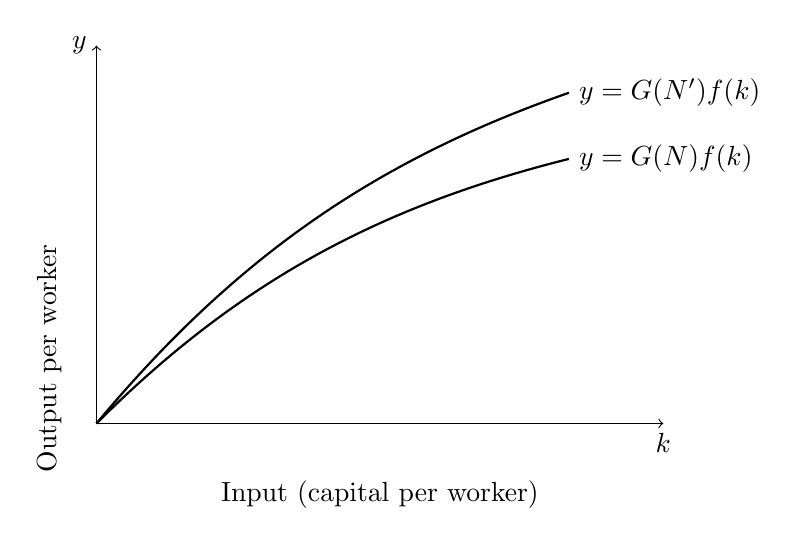
\begin{tikzpicture}[scale=1.2]
    % Axes
    \draw[->] (0,0) -- (6,0) node[below] {$k$};
    \draw[->] (0,0) -- (0,4) node[left] {$y$};
    
    % Axes labels
    \node[below] at (3,-0.5) {Input (capital per worker)};
    \node[rotate=90, left] at (-0.5,2) {Output per worker};
    
    % Production functions
    \draw[thick] (0,0) .. controls (1.5,1.5) and (3,2.3) .. (5,2.8) node[right] {$y = G(N)f(k)$};
    \draw[thick] (0,0) .. controls (1.5,1.8) and (3,2.8) .. (5,3.5) node[right] {$y = G(N')f(k)$};
    
\end{tikzpicture}

\end{document}